\documentclass[a4paper,10pt]{ctexbook}
\usepackage{amsfonts}
\usepackage{bbm}
\usepackage{mathrsfs}
\usepackage{amsfonts}
\usepackage{graphicx}
%\input amssymb.sty
 %\usepackage[notref,notcite]{showkeys}
 \usepackage{mathrsfs,amsfonts,amsmath,amssymb}
%\usepackage[dvips]{color}
\usepackage{color}
 \usepackage{amssymb}
 \usepackage{amsthm}
\usepackage{CJK}
\usepackage{CJK,CJKnumb}
\usepackage[final]{pdfpages}
\usepackage{fancyhdr}
%\usepackage{actuarialsymbol}


\allowdisplaybreaks
 \setlength{\topmargin}{0cm}
 \setlength{\oddsidemargin}{0.0cm}
 \setlength{\evensidemargin}{0.0cm}
 \setlength{\textwidth}{15cm}
 \setlength{\textheight}{20cm}
 \setlength{\parindent}{0.85cm}
 \setlength{\parskip}{4pt}
\def\red{\color{red}}
\def\blue{\color{blue}}
 \renewcommand\baselinestretch{1.2}



\newcommand{\song}{\CJKfamily{song}}    % 宋体
\newcommand{\fs}{\CJKfamily{fs}}        % 仿宋体
\newcommand{\kai}{\CJKfamily{kai}}      % 楷体
\newcommand{\hei}{\CJKfamily{hei}}      % 黑体
\newcommand{\li}{\CJKfamily{li}}        % 隶书
\newcommand{\you}{\CJKfamily{you}}      % 幼圆





 \def\qed{\hfill$\Box$\medskip}
 \def\rto{\rightarrow\infty}
 \def\z{\left}
 \def\y{\right}
 \def\no{\nonumber}
 \def\mbe{\mathbb{E}}
 \def\mbp{\mathbb{P}}
 \def\ka{{\kappa_1}}
\usepackage{indentfirst}

%\DeclareRobustCommand{\actuarial}[2][]{%
%\def\arraystretch{0}%
%\setlength\arraycolsep{0.5pt}%
%\setlength\arrayrulewidth{0.5pt}%
%\setbox0=\hbox{$\scriptstyle#1#2$}%
%\begin{array}[b]{*2{@{}>{\scriptstyle}c}|}
%\cline{2-2}%
%\rule[1.25pt]{0pt}{\ht0}%
%#1 & #2%
%\end{array}%
%}


\DeclareRobustCommand{\annu}[1]{_{%
\def\arraystretch{0}%
\setlength\arraycolsep{1pt}% adjust these
\setlength\arrayrulewidth{.2pt}% two settings
\begin{array}[b]{@{}c|}\hline
\\[\arraycolsep]%
\scriptstyle #1%
\end{array}%
}}




\begin{document}

\theoremstyle{definition}\newtheorem{definition}{\noindent\mbox{\bf\hei 定义}}[chapter]
\newtheorem{assumption}{\noindent\mbox{Assumption}}[chapter]
\theoremstyle{remark} \newtheorem{remark}{\noindent\mbox{\bf\hei 注}}[chapter]
\newtheorem{exs}{\noindent\mbox{\bf\hei 作业}}[chapter]
\theoremstyle{remark}\newtheorem{example}{\noindent\mbox{\bf\hei 例}}[chapter]
\newtheorem{lemma}{\noindent\mbox{\bf\hei 引理}}[chapter]
\newtheorem{theorem}{\noindent\mbox{\bf\hei 定理}}[chapter]
\newtheorem{proposition}{\noindent\mbox{\bf\hei 命题}}[chapter]
\newtheorem{corollary}{\noindent\mbox{\bf\hei 推论}}[chapter]
%%%%%%%%%%%%%%%%%%%%%%%%55

\def\proof{\noindent{\bf\hei 证明.~~}}



%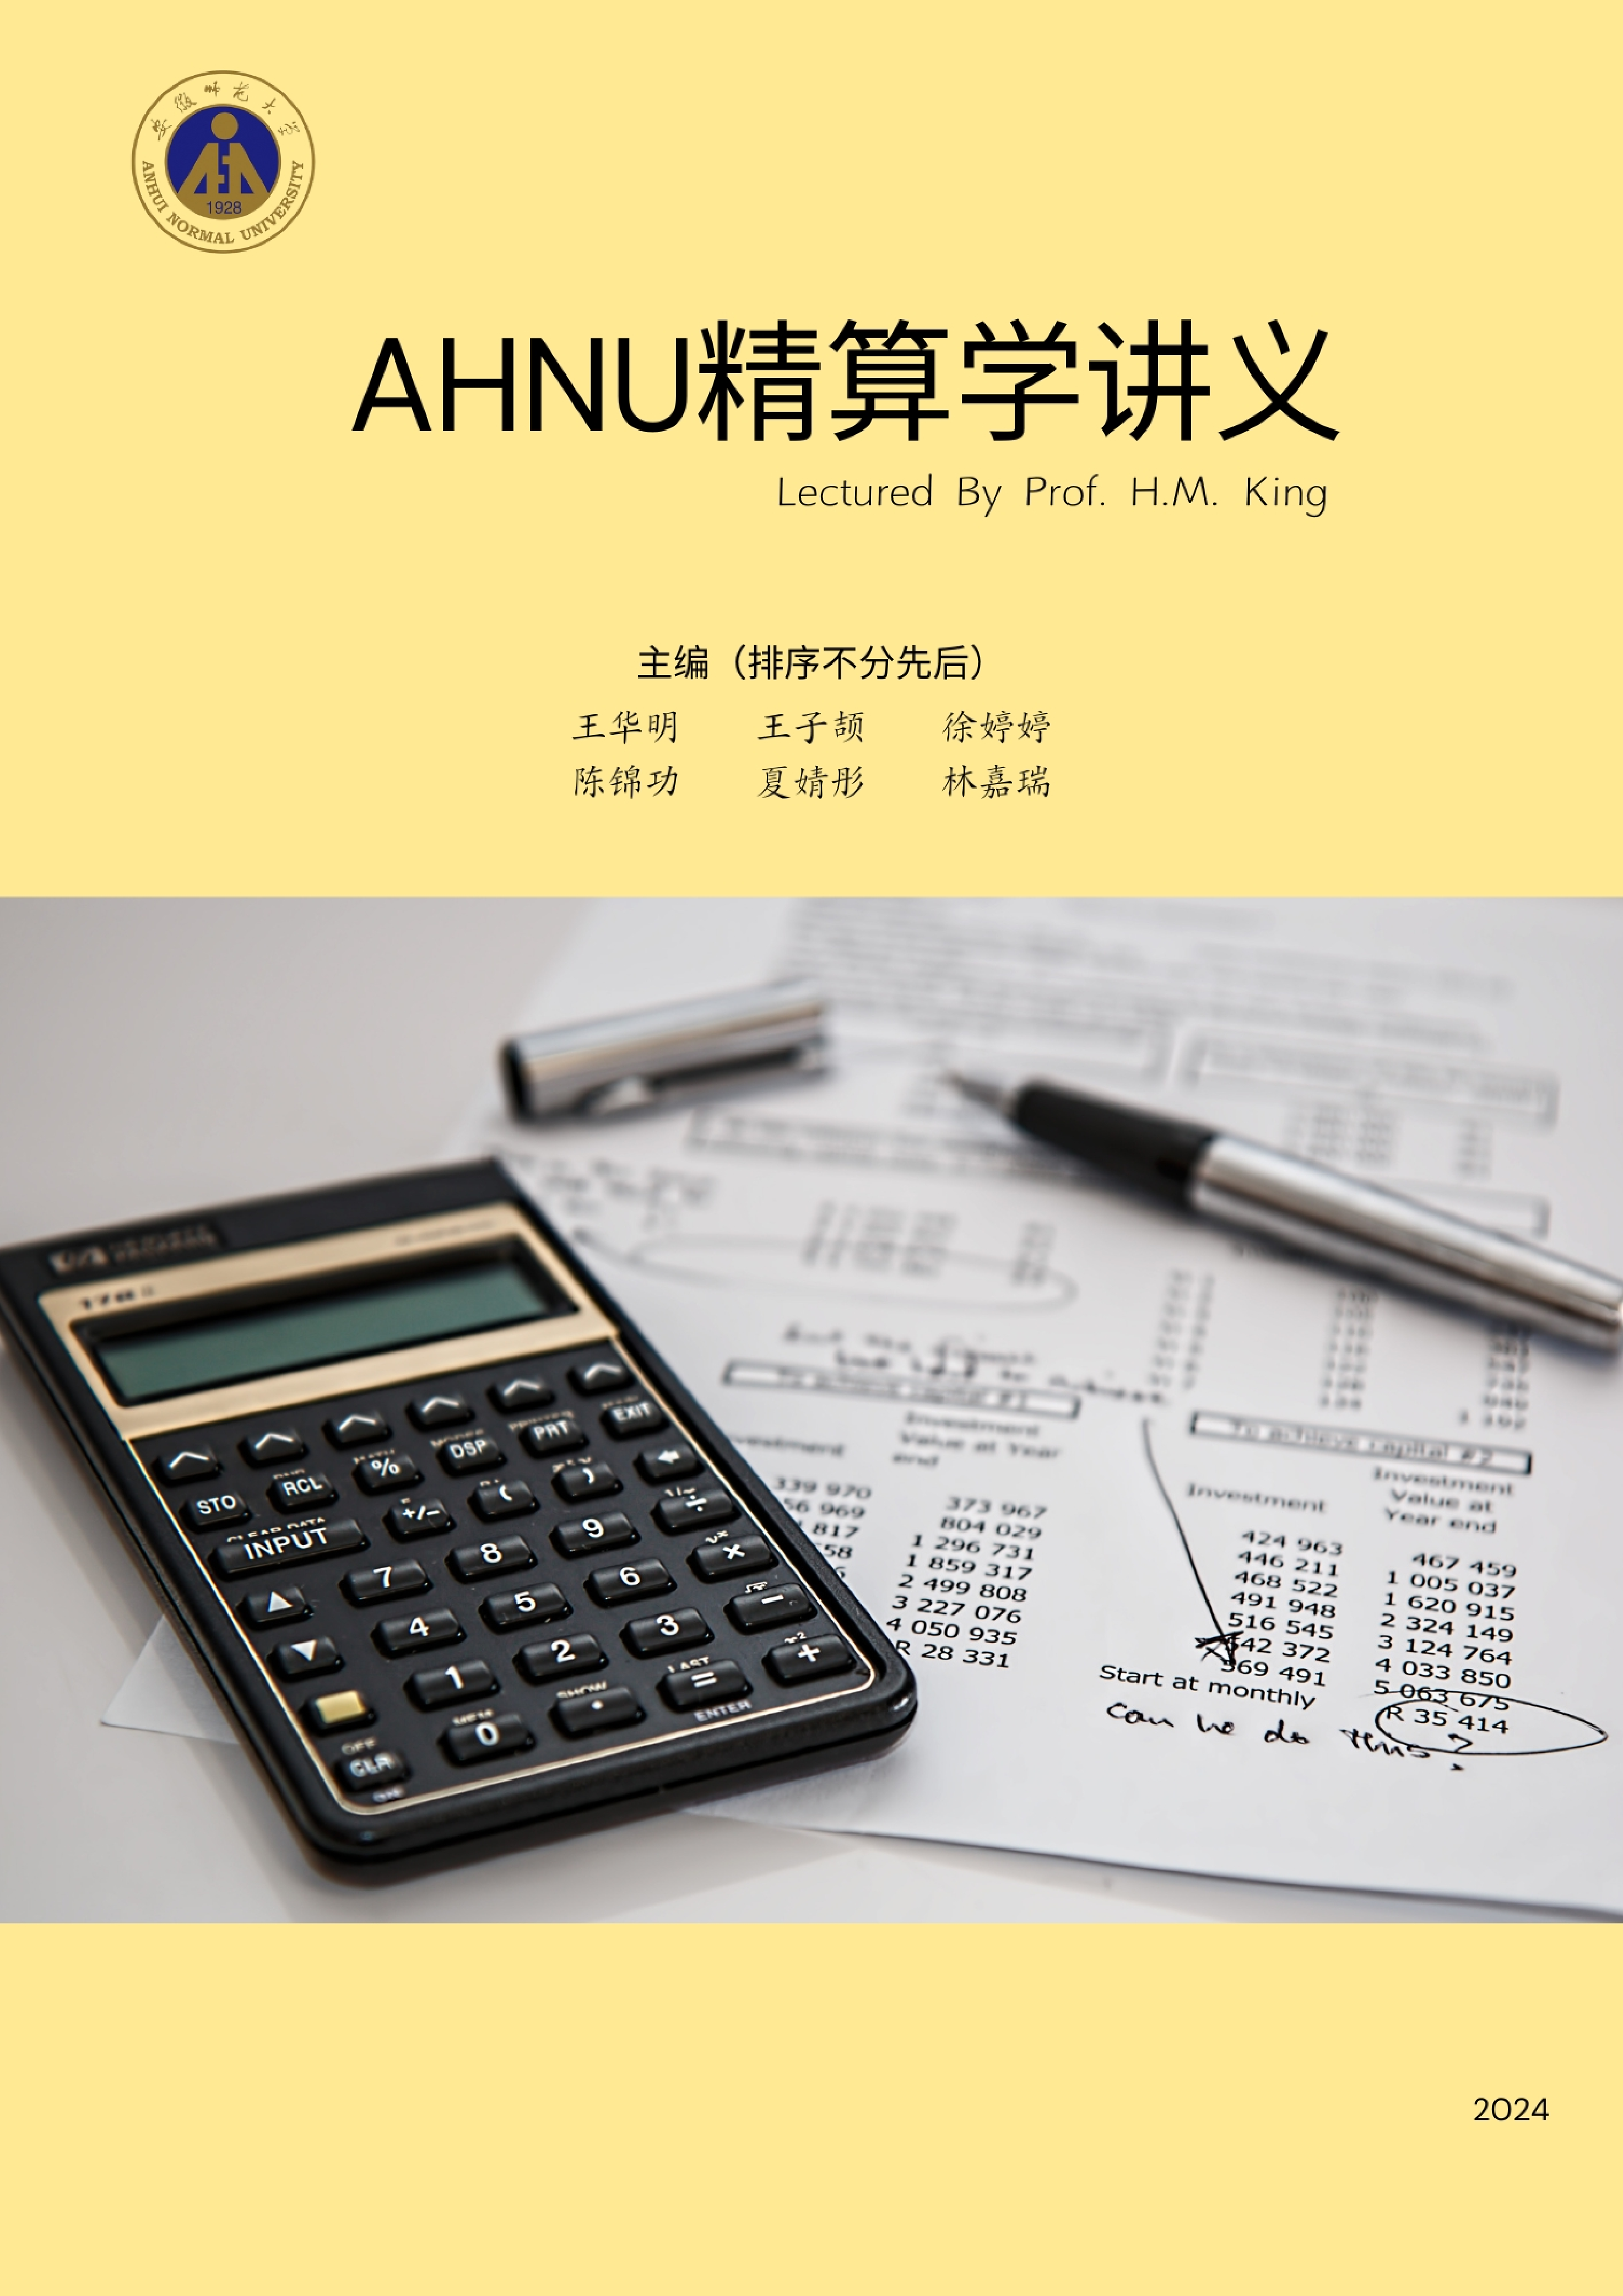
\includepdf{PDFCover.pdf}

%\large
\title{\Huge\textbf{《精算学》讲义}\footnote{本讲义由陈锦功、王子颉、林嘉瑞、夏婧彤、徐婷婷等几名同学协助录入.}}

\author{王华明\thanks{安徽师范大学数学与统计学院, 安徽芜湖(241003).  Email:hmking@ahnu.edu.cn}}
\date{}
\frontmatter
\maketitle

\vspace{-6mm}

\large
\begin{center}
    \begin{minipage}[c]{12cm}
        \begin{center}\textbf{序}\quad \end{center}
        \vspace{-0em} \hspace{2em} 本讲义是王华明老师在2023-2024年第2学期讲授的《精算学》课程笔记的电子版. 授课对象包括安徽师范大学2021级统计学专业全体同学及少数几位跨专业选课的同学. 教材选用的是北京大学出版社的《寿险精算基础》一书, 该书的作者是杨静平教授. 在此对北京大学出版社及杨静平教授表示感谢.

    \end{minipage}
\end{center}

%\tableofcontents
%\newpage


%\newpage
%% \pagestyle{empty}
%\section*{更新日志}
%2024.2.28
%
%由H.M. King老师领导的编写组成立,由WZJ和LJR完成了初步模板的编写。
\newpage

\begin{center}
    {\bf\hei 精算学内容}
\end{center}
\begin{enumerate}
    \item 你能活多久?(生存分布)
    \item 你死的时候, 保险公司支付你1元, 这1元的现值为多少?(人寿保险)
    \item 在你活着时, 保险公司每年支付你1元, 这些支付的现值是多少?(生存年金)
    \item 上述的寿险与生存年金, 你该向保险公式缴纳多少保费?(保费理论)
    \item 保险公司为了保证支付, 要准备多少钱?(准备金理论)
\end{enumerate}
\newpage
\thispagestyle{empty}

\mainmatter
\chapter{生存分布}
\section{新生儿的生存分布}
\begin{itemize}
    \item[{\bf\hei 一.}]{\bf\hei 生存函数}
\end{itemize}

设有一个新生儿, 其寿命记为$X,$ 则$X$是一个非负随机变量. 假设$X$为一个连续型随机变量, 其分布函数为$F_X(x),$ 密度函数为$f_X(x).$ 回忆一下, 我们有 $F_X(x)=\int_0^x f_X(t)dt$ 且在$f_X(x)$的连续点上有
$$F_X'(x)=f_X(x).$$
如下我们总假设密度函数$f_X(t)$连续.
\begin{definition}
    称$s(t):=P(X>t),t>0$ 为$X$的生存函数.
\end{definition}
易知
\begin{align}\label{sf}
    s(t)=1-F_X(t), s'(t)=-f_X(t).
\end{align}

\begin{itemize}
    \item[{\bf\hei  二.}]{\bf\hei 死亡力}
\end{itemize}
现欲刻画一个$t$时刻还活着的个体瞬间死去的可能性, 做如下计算:

\begin{align}\label{swl}
    \lim_{h\downarrow0} & \frac{P(t<X\le t+h|X>t)}{h}=\lim_{h\downarrow0} \frac{P(t<X\le t+h)}{hP(X>t)}\no                                            \\
                        & =\lim_{h\downarrow0}\frac{P(X\le t+h)-P(X\le t)}{hP(X>t)}=\lim_{h\downarrow0}\frac{F_X(t+h)-F_X(t)}{h}\frac{1}{1-F_X(t)}\no \\
                        & =\frac{F_X'(t)}{1-F_X(t)}=\frac{f_X(t)}{1-F_X(t)}=-\frac{s'(t)}{s(t)}.
\end{align}

\begin{definition}
    称$\mu(t):=-\frac{s'(t)}{s(t)},t\ge 0$ 为新生儿的死亡力函数.
\end{definition}
由\eqref{swl}中的计算可知, 死亡力$\mu(t)$刻画了新生儿在$t$附近死去的``快慢".

\begin{proposition} 关于$\mu(t),$ $s(t)$ 及 $f_X(t)$ 有如下结论:

    {\rm\bf(i)} $\mu(t)=-\frac{s'(t)}{s(t)}=\frac{f_X(t)}{1-F_X(t)}=\frac{f_X(t)}{s(t)};$

    {\rm\bf(ii)} $f_X(t)=\mu(t)s(t);$

    {\rm\bf(iii)} $s(t)=e^{-\int_0^t\mu(s)ds}.$

\end{proposition}
\proof (i)和(ii)可由死亡力$\mu(t)$的定义及(1)式直接得出. 现证明(iii). 注意到$s(0)=P(X>0)=1$及
$$\mu(t)=-\frac{s'(t)}{s(t)}=-[\ln s(t)]'.$$ 所以有
$$\ln s(t)=-\int_0^t\mu(s)ds.$$ 故$s(t)=e^{-\int_0^t\mu(s)ds},$ (iii) 得证. \qed


\begin{remark}
    \begin{enumerate}
        \item[{\bf(a)}] 由$s(t) = e^{-\int_{0}^{t}\mu(s)\mathrm{d}s}$及$ \mu(t) = -\frac{s'(t)}{s(t)}$ 可知, 生存函数$s(t)$ 与死亡力函数$\mu(t)$ 相互唯一确定.
        \item[{\bf(b)}] 一个函数$\mu(t)$要作为死亡力, 必须满足以下两条:
            \begin{enumerate}
                \item[ $ 1^\circ$] $\mu(t) \geq 0, ~\forall t \geq 0$ (保证$s(t)$单调递减).
                \item[$2^\circ$] $\int_0^{\infty}\mu(t)\mathrm{d}t = \infty$(保证$s(\infty)=0$).
            \end{enumerate}
    \end{enumerate}

\end{remark}




\begin{example}
    假设新生儿的寿命服从以$\lambda$为参数的指数分布, 则密度函数$f_X(t)=\lambda e^{-\lambda x},x>0.$ 分布函数$F_X(t)=\int_0^t f_X(s)ds=1-e^{-\lambda t}, t>0.$ 生存函数$s(t)=1-F_X(t)=e^{-\lambda t},t>0.$  故其死亡力函数为
    \begin{align}\label{ep}
        \mu(t)=-\frac{s'(t)}{s(t)}=-\frac{-\lambda e^{-\lambda t}}{e^{\lambda t}}\equiv\lambda.
    \end{align}
\end{example}

\begin{remark}
    由\eqref{ep}式可知, 若新生儿寿命服从以$\lambda$ 为参数的指数分布, 则死亡力$\mu(t)\equiv \lambda,$ 和$t$无关. 这表示新生儿的死亡力在任何时候都是一样的. 也就是说, 新生儿永远年轻. 这当然与实际情况不符. 所以, 指数分布作为寿命分布是有缺陷的. 但由于指数分布的计算较为简单, 所以在理论研究中, 学者们很多时候都采用指数分布作为寿命分布.
\end{remark}
\begin{itemize}
    \item[{\bf\hei 三.}]{\hei\bf 整数年龄与分数年龄}
\end{itemize}
很多时候, 保险金都是在整数时刻支付的. 所以有必要研究整数年龄和分数年龄. 设$K(0)$为$X$的整数部分, $S(0)$为$X$的分数部分. 即
$$X = K(0) + S(0).$$
记$\mathring{e}_0 = E(X),$ 它表示新生儿的期望寿命; 记$e_0 = E(K(0)),$ 它表示期望整数寿命. 易知
\begin{equation*}
    e_0 \le \mathring{e}_0 < e_0 + 1.
\end{equation*}

\begin{lemma}\label{lemm0}
    设随机变量$X$的$n$阶矩存在, 即$E(X^n) < \infty,$ 则$\lim_{M \rightarrow \infty}M^ns(M) = 0.$
\end{lemma}
\begin{proof} 注意到
    \begin{align}
        E(X^n)=\int_{0}^\infty s^n f_X(s)ds=\int_0^Ms^n f_X(s)ds +\int_{M}^\infty s^n f_X(s)ds.
    \end{align}
    因$X$的$n$阶矩存在, 故上式左右两端都是有限的. 由于 $\lim_{M\rto} \int_0^Ms^n f_X(s)ds=E(X^n),$ 所以
    $\lim_{M\rto}\int_{M}^{\infty} s^nf_X(s)\mathrm{d}s=0.$ 于是
    \begin{align}
        M^n s(M) & = M^nP(X>M)
        =    \int_{M}^{\infty} M^nf_X(s)\mathrm{d}s  \no                                 \\
                 & \leq \int_{M}^{\infty} s^nf_X(s)\mathrm{d}s \rightarrow 0,\ M\rto.\no
    \end{align}
    引理证毕. \qed
\end{proof}

\begin{proposition}如下结论成立:
    \begin{enumerate}
        \item[(1)] $\mathring{e}_0 = E(X) = \int_0^{\infty}s(t)\mathrm{d}t;$
        \item[(2)] $E(X^2) = \int_{0}^{\infty} 2ts(t)\mathrm{d}t;$
        \item[(3)] $E(K(0)^2) = \sum_{n = 1}^{\infty} (2n-1)s(n);$
        \item[(4)] $e_0=E(K(0)) = \sum_{n = 1}^{\infty} s(n).$
    \end{enumerate}
\end{proposition}
\begin{proof}由分部积分公式和引理\ref{lemm0}可知
    \begin{equation*}
        \begin{aligned}
            {E}\left(X^{n}\right) & =\int_0^\infty t^n\mathrm{d}F(t)=\lim_{M\to\infty}\int_0^Mt^n\mathrm{d}F(t)=-\lim_{M\to\infty}\int_0^Mt^n\mathrm{d}s(t) \\
                                  & \left.=-\lim_{M\to\infty}(\left[t^ns(t)\right]\right|_0^M-\int_0^Mnt^{n-1}s(t)\mathrm{d}t)                              \\
                                  & =\lim_{M\to\infty}[-M^ns(M)]+\lim_{M\to\infty}\int_0^Mnt^{n-1}s(t)\mathrm{d}t                                           \\
                                  & =\int_0^\infty nt^{n-1}s(t)\mathrm{d}t.
        \end{aligned}
    \end{equation*}
    故(1)与(2)得证. 下证(3), 由离散型随机变量函数期望的计算公式, 有
    \begin{align*}
        E(K(0)^2) & = \sum_{k = 0}^{\infty} k^2P(K(0) = k)
        = \sum_{k = 0}^{\infty} k^2[P(X \geq k) - P(X \geq k+1)]                                                            \\
                  & = \sum_{k = 0}^{\infty} k^2s(k) - \sum_{k = 0}^{\infty} k^2s(k+1)                                       \\
                  & =\sum_{k = 0}^{\infty} k^2s(k) - \sum_{k = 0}^{\infty} (k+1)^2s(k+1)+\sum_{k = 0}^{\infty} (2k+1)s(k+1) \\
                  & = \sum_{k = 0}^{\infty} (2k+1)s(k+1)                              = \sum_{n = 1}^{\infty} (2n-1)s(n).
    \end{align*}
    故(3)得证. 类似可证(4). \qed
\end{proof}

\section{$x$岁个体的生存分布}

\begin{itemize}
    \item[{\bf\hei 一.}]{\bf\hei $x$岁个体余命的分布、密度及生存函数}
\end{itemize}

为了方便, 今后将一个$x$岁还活着的个体记为$(x).$ 个体$(x)$的余命记为$T(x).$ 显然有
$$T(x)=X-x.$$
这里特别强调一下,
$T(x)$的分布表示在已知事件$\{X>x\}$发生的条件下, $X-x$的分布. 如果新生儿在$x$岁之前死了, 也就没有了所谓的个体$(x),$ 其余命也就无从谈起.

记$F_{T(x)}(t)$为$T(x)$的分布函数, 则
\begin{align}\label{ft}
    F_{T(x)}(t) & = P(T(x) \leq t|X > x)
    = P(X- x \leq t | X > x)\no                        \\
                & = \frac{P(x<X \leq t + x)}{P(X > x)}
    = \frac{P(X > x) - P(X > x + t)}{P(X > t)}\no      \\
                & = 1 - \frac{s(x+t)}{s(x)}.
\end{align}
记$f_{T(x)}(t)$为$T(x)$的密度函数, 则
\begin{equation}\label{ftd}
    f_{T(x)}(t) = F_{T(x)}'(t) = -\frac{s'(x+t)}{s(x)} = \frac{f_X(x+t)}{s(x)}.
\end{equation}
\begin{definition}
    称$s_{T(x)}(t): = P(T(x)>t)$为个体 $(x)$的的生存函数.
\end{definition}

由\eqref{ft}可得
\begin{align}\label{stf}
    s_{T(x)}(t)=1-F_{T(x)}(t)=\frac{s(x+t)}{s(x)} \text{ 且 }\  s_{T(x)}'(t)=-f_{T(x)}(t).
\end{align}


\begin{itemize}
    \item[{\bf\hei 二.}]{\bf\hei $x$岁个体的死亡力}
\end{itemize}
为了解个体$(x)$在$x+t$岁附近死去的``快慢", 考虑极限

\begin{align*}
    \lim_{\Delta t\to0+} & \frac{P(t<T(x)\leqslant t+\Delta t|T(x)>t)}{\Delta t}
    =  \lim_{\Delta t\to0+}\frac{P(t<T(x)\leqslant t+\Delta t)}{\Delta tP(T(x)>t)}                                          \\
                         & = \lim_{\Delta t\to0+}\frac{s_{T(x)}(t) - s_{T(x)}(t + \Delta t)}{\Delta t}\frac{1}{s_{T(x)}(t)}
    = - \frac{s_{T(x)}'(t)}{s_{T(x)}(t)}                                                                                    \\
                         & = - \frac{\frac{s'(x+t)}{s(x)}}{\frac{s(x+t)}{s(x)}}
    =  -\frac{s'(x+t)}{s(x+t)} = \mu(x+t).
\end{align*}

\begin{definition}
    称$\mu_x(t) = -\frac{s_{T(x)}'(t)}{s_{T(x)}(t)}$为$X$岁个体在$t$年后的死亡力函数。
\end{definition}

\begin{proposition}\label{p21} 我们有

    {\bf(i)} $s_{T(x)}(t)=1-F_{T(x)}(t)=\frac{s(x+t)}{s(x)};$

    {\bf(ii)} $\mu_{x}(t)=\frac{f_{T(x)}(t)}{1-F_{T(x)}(t)}=\frac{f_{T(x)}(t)}{s_{T(x)}(t)}=-\frac{s_{T(x)}'(t)}{s_{T(x)}(t)}.$

    {\bf(iii)} $f_{T(x)}(t)=s_{T(x)}(t)\mu_{x}(t);$

    {\bf(iv)} $\mu_x(t)=\mu(x+t);$

    {\bf(v)} $s_{T(x)}(t)=e^{-\int_0^t \mu_x(s)ds}=e^{-\int_0^t \mu(x+s)ds}=e^{-\int_x^{x+t} \mu(s)ds}.$

\end{proposition}
\proof 利用\eqref{ft}, \eqref{ftd} 和 \eqref{stf}, 很容易证明 (i), (ii), (iii). 下证(iv). 由(ii), \eqref{ftd} 及\eqref{stf} 可得,
\begin{align*}
    \mu_{x}(t)=\frac{f_{T(x)}(t)}{s_{T(x)}(t)}=\frac{f_{X}(x+t)/s(x)}{s(x+t)/s(x)}=\frac{f_{X}(x+t)}{s(x+t)}=\mu(x+t).
\end{align*}
其中, 为了得到最后一个等号, 我们用了命题1.1中的第一条. (iv)得证.

最后证明(v). 注意到$s_{T(x)}(0)=P(T(x)>0)=1$ 且由第(ii)条有
$$\mu_{x}(t)=-\frac{s_{T(x)}'(t)}{s_{T(x)}(t)}=-[\ln s_{T(x)}(t)]'.$$
故 $\ln s_{T(x)}(t)=-\int_0^t\mu_x(s)ds.$ 从而
$s_{T(x)}(t)=e^{-\int_0^t\mu_x(s)ds}.$ 又因为$\mu_x(t)=\mu(x+t),$ 故
\begin{align*}
    s_{T(x)}(t)=e^{-\int_0^t\mu_x(s)ds}=e^{-\int_0^t\mu(x+s)ds}=e^{-\int_x^{x+t} \mu(s)ds},
\end{align*}
其中, 为得到最后一个等号, 我们用定积分的换元法即可. \qed


\begin{remark}
    理论上, 一个人一旦出生, 其死亡力就``注定"了. 如果他在$x$岁还活着, 在$t$ 年后他变为$x+t$ 岁, 此时他的死亡力是$\mu_x(t).$ 换一种观点, 如果站在0 时刻(他出生时)看, 他在$x+t$岁的死亡力应为$\mu(x+t).$ 故有
    $$\mu_x(t)=\mu(x+t).$$
\end{remark}

\begin{example}
    设新生儿的寿命服从以$\lambda>0$ 为参数的指数分布. 则
    $s(t)=e^{-\lambda t}, t>0.$ 从而有
    \begin{align*}
         & F_{T(x)}(t)=1-\frac{s(x+t)}{s(x)}=1-\frac{e^{-\lambda(x+t)}}{e^{-\lambda x}}=1-e^{-\lambda t} =F_X(t); \\
         & f_{T(x)}(t)=F_{T(x)}'(t)=F_X'(t)=f_X(t);                                                               \\
         & \mu_x(t)=\mu(x+t)\equiv\lambda.
    \end{align*}
    以上计算再次表明, 在指数分布寿命假设下, 新生儿的的寿命$X$与$x$岁的个体的余命$T(x)$的分布相同. 进一步说明指数分布作为寿命分布是有缺陷的.
\end{example}


\begin{proposition}$\forall u,t>0,$ 有
    \begin{align}
         & P(T(x)>t+u|T(x)>t)=P(T(x+t)>u).\label{tu}
    \end{align}
    该式的含义为: 一个$x$岁的人, 在$x+t$岁还活着的条件下, 再活$u$年不死的概率与一个$x+t$岁的人再$u$年内未死的概率相等.
\end{proposition}

\proof 对$u,t>0,$ 由条件概率定义知
\begin{align*}
    P(T(x) & >t+u|T(x)>t)=\frac{P(T(x)>t+u)}{P(T(x)>t)}=\frac{P(X-x)>t+u}{P(X-x)>t} \\
           & =\frac{P(X-(x+t)>u)}{P(X>x+t)}=  P(X-(x+t>u|X>x+t))                    \\
           & =P(T(x+t)>u)=\frac{P(T(x)>t+u)}{P(T(x)>t)}.
\end{align*}
命题证毕. \qed

\begin{remark}由\eqref{tu}式立即可得
    \begin{align}\label{tul}
         & P(T(x)\leq t+u|T(x)>t)=P(T(x+t)\leq u).
    \end{align}
\end{remark}
\begin{example}
    设新生儿的寿命服从指数分布,参数为$\lambda$,则$\mu(t)\equiv\lambda,$
    \begin{align*}
         & s(t)=e^{-\lambda t},t>0.                                                                                       \\
         & F_{T(x)}=1-\frac{s(x+t)}{s(x)}=1-e^{- \lambda t}=F_x(t).                                                       \\
         & f_{T(x)}(t)=F_{T(x)}(t)=\lambda e^{- \lambda t}=f_x(t),t>0.                                                    \\
         & s_{T(x)}(t)=\frac{s(x+t)}{s(x)}=e^{-\lambda t}=s(t),t>0.                                                       \\
         & \mu_x(t)=\mu(x+t)\equiv\mu,t>0.                                                                                \\
         & e_x = \sum_{k=1}^{\infty} {_kp_x}=\sum_{k=1}^{\infty} {e^{- \lambda t}}=\frac{e^{- \lambda}}{1-e^{- \lambda}}. \\
         & \mathring{e}_x=\int_{0}^{\infty}{_tp_x}dt=\int_{0}^{\infty}{e^{- \lambda t}}dt=\frac{1}{\lambda}.
    \end{align*}
    显而易见, 这里的$\mathring e_x $和$e_x$与$x$无关, 也就是说,  所有人的剩余寿命的期望都是一样的, 和他现在的年龄无关. 这进一步说明指数分布作为寿命分布是有缺陷的.   此外, 因$\mathring{e}_x=ET(x)=\frac{1}{\lambda},$ 故指数分布的参数$\lambda$正好是期望寿命的倒数.
\end{example}

\begin{itemize}
    \item[{\bf\hei 三.}]{\bf\hei 一些精算学表示法}
\end{itemize}
注意到 $ S_{T(x)}(t)=P(T(x)>t)$表示个体$ (x)$在$t$年后还活着的概率; 而$F_{T(x)}(t)=P(T(x)\le t)$表示个体$(x)$在$t$年内死去的概率. 这些记号都很复杂, 书写比较困难. 故精算学中需引入一些简单的记号.


定义如下几个记号:
\begin{enumerate}
    \item[$\mathring 1.$] 用$_tp_{x}\stackrel{\text{def}}{=}P(T(x)>t)=S_{T(x)}(t)$
        表示个体$(x)$在$t$年后还活着的概率. 显然有
        $$ {}_tP_x=S_{T(x)}(t)=\mathrm{e}^{-\int_{0}^{t}\mu_x(s)\mathrm{d}s}=\mathrm{e}^{-\int_{0}^{t}\mu(x+s)\mathrm{d}s}=\mathrm{e}^{-\int_{x}^{x+t}\mu(s)\mathrm{d}s}.$$
    \item[$\mathring 2.$] 用$_tq_{x}\stackrel{\text{def}}{=}P(T(x\leq t)=F_{T(x)}(t))$
        表示一个$x$岁的人在$t$年内死亡的概率. 易知
        $$_tp_{x}+{}_tq_{x}=1.$$
    \item[$\mathring 3.$] 用$ _{u|t}q_x=P(u<T(x)\leq u+t)$
        表示一个$x$岁的人在$x+u$岁还活着, 但在未来$t$年内死亡的概率.
\end{enumerate}
\begin{proposition}如下几个结论成立:

    (i) $\frac{d(_tp_x)}{dt}=-_tp_x\mu_x(t);$

    (ii) $\frac{d(_tp_x)}{dx}=-_tp_x(\mu(x)-\mu(x+t)).$


\end{proposition}

\proof (i) 注意到${}_tp_x=\mathrm{e}^{-\int_{0}^{t}\mu_x(s)ds}.$ 故
$$\frac{d(_tp_x)}{dt}=\frac{d(\mathrm{e}^{-\int_{0}^{t}\mu_x(s)ds})}{dt}=\mathrm{e}^{-\int_{0}^{t}\mu_x(s)ds}({-\int_{0}^{t}\mu_x(s)ds})^{\prime}_t=-_tp_x\mu_x(t).$$

(ii) 利用等式${}_tp_x=e^{-\int_{x}^{x+t}\mu_x(s)ds},$ 有
$$\frac{d(_tp_x)}{dx}=(e^{-\int_{x}^{x+t}\mu_x(s)ds})^{\prime}=e^{-\int_{x}^{x+t}\mu(s)ds}({-\int_{x}^{x+t}\mu(s)ds})^{\prime}_x=-_tp_x(\mu(x)-\mu(x+t)).$$
命题证毕.
\qed

\begin{proposition}以下结论成立:

    (1) $f_{T(x)}(t)=_tp_x*\mu_x(t);$

    (2) $_tp_x={}_sp_x\cdot{}_{t-s}p_{x+s},0\leq s\leq t;$

    (3) ${}_{u|t}q_x=_up_x-_{u+t}p_x, u,t>0;$

    (4) ${}_{u|t}q_x=_up_x{}_{t}q_{x+u},u,t\ge0.$
\end{proposition}
\proof (1)是显然的, 不需证明. (2)
固定$0\le s\le t,$ 则由条件概率性质可知
\begin{align*}
    {}_tp_x & =P(T(x)>t)=P(T(x)>s)P(T(x)>t|T(x)>s) \\
            & ={}_sp_xP(T(x)>t+s-s|T(x)>s)         \\
            & ={}_sp_xP(T(x+s)>t-s)                \\
            & ={}_sp_x\cdot{}_{t-s}p_{x+s}.\end{align*}

(3) 对$t,u\ge0,$ 简单计算可知
\begin{align*}
    {}_{u|t}q_x & =P(u<T(x)\leq u+t)                          \\
                & =P(T(x)>u)-P(T(x)>u+t)={}_up_x-{}_{u+t}p_x.
\end{align*}

(4) 固定$t,u\ge0,$ 利用\eqref{tul}得
\begin{align*}
    {}_{u|t}q_x & =P(u<T(x)\leq u+t)=P(T(x)>u)P(T(x)\leq u+t|T(x)>u) \\
                & ={}_up_xP(T(x+u)<t)= {}_up_x{}_{t}q_{x+u}.
\end{align*}
命题证毕. \qed

\begin{itemize}
    \item[{\bf\hei 四.}]{\bf\hei 个体$(x)$的整数与分数余命}
\end{itemize}
类似处理新生儿的寿命一样, 可将个体$(x)$的余命$T(x)$分为整数部分和小数部分.
设
\begin{align*}
     & T(x)=K(x)+S(x)
\end{align*}
其中$K(x)$是$T(x)$的整数部分, $S(x)$是$T(x)$的小数部分. 记
\begin{align*}
     & \mathring{e_x}\stackrel{\text{def}}{=}E(T(x)), \   {e_x}\stackrel{\text{def}}{=}E(K(x))
\end{align*}
则简单计算可知 \begin{align*}
    \mathring{e_x} & =E(T(x))=\int_{0}^{\infty}P(T(x)>t)d t=\int_{0}^{\infty}{_tp_xdt};                      \\
    {e_x}          & =E(K(x))=\sum_{k=0}^{\infty}kP(K(x)=k)                                                  \\
                   & =\sum_{k=0}^{\infty}k[P(T(x)\geq k)-P(T(x)\geq k+1)]                                    \\
                   & =\sum_{k=0}^{\infty}k_kp_x-\sum_{k=0}^{\infty}k_{k+1}p_x=\sum_{k=0}^{\infty}{_{k+1}p_x} \\
                   & =\sum_{k=0}^{\infty}{_kp_x}.
\end{align*}






\section{随机生存群}
\begin{itemize}
    \item[{\bf\hei 一.}]{\bf\hei 模型描述}
\end{itemize}

设0时刻系统中有$l_0$个新生儿, 他们的寿命独立同分布, 服从某分布, 生存函数为$s(t),t\ge 0.$  记

$\mathscr{L}(x)$ 为在$x$ 岁还活着的总人数;

$_t \mathscr{D}_x$为$[x,x+t]$内死去的总人数.

设系统中初始时刻的$l_0$个人的寿命分别为$X_1,X_2,…,X_n$, 则他们独立同分布, 且
$$P(X_i>t)=s(t), i=1,...,n.$$
显然有
\begin{align*}
     & \mathscr{L}(x)=\sum_{i=1}^{\iota_{\mathrm{0}}}I_{\{X_{i}\geqslant x\}},\ {}_t\mathscr{D}_x=\sum_{i=1}^{l_0}I_{\{ x\leqslant X_i<x+t\}}
\end{align*}
其中
$
    I_{A}=\left\{\begin{array}{ll}1,&\omega\in A,\\0,&\omega\in A^c\end{array}\right.
$ 为示性函数.

令 \begin{align*}
    l_x     & \overset{def}{=}E\z(\mathscr L(x)\y), \text{ 它表示在}x\text{岁还活着的期望人数};         \\
    {}_td_x & \overset{def}{=}E\z({}_t\mathscr D_x \y),\text{ 它表示在}[x,x+t)\text{内死去人数的期望}.
\end{align*}



\begin{itemize}
    \item[{\bf\hei 二.}]{\bf\hei 几个结论}
\end{itemize}

\begin{proposition} 如下结论成立:
    $$l_x=l_0s(x),\ {}_td_x=l_x-l_{x+t}.$$
\end{proposition}
\proof 注意到$E(I_A)=P(A),$ 所以
\begin{align*}
    l_x     & =E(\mathscr{L}(x))=E(\sum_{k=0}^{l_0}I_{\{x_k>x\}})                        \\
            & =\sum_{k=0}^{l_0}E(I_{\{x_k>x\}})
    =\sum_{k=1}^{l_0}P(X_k>x)
    =\sum_{k=1}^{l_0}P(X_1>x)                                                            \\
            & =l_0P(X_1>x)=l_0s(x);                                                      \\
    {}_td_x & =E(_t\mathscr{D}_t)=E(\sum_{k=1}^{l_0}I_{\{x<x_k\leq x+t\}})               \\
            & =\sum_{k=1}^{l_0}E(I_{\{x<x_k\leq x+t\}})=\sum_{k=1}^{l_0}E(x<x_k\leq x+t) \\
            & =l_0P(x<X_1\leq x+t)=l_0[P(X_1>x)-P(X_1>x+t)]                              \\
            & =l_0s(x)-l_0s(x+t)
    =l_x-l_{x+t}.
\end{align*}

引入$l_x$及${}_td_x$的目的是为了计算生存概率${}_tp_x$与死亡概率${}_tq_x.$
\begin{proposition}如下结论成立:

    (i) ${}_tp_x=\frac{l_{x+t}}{l_x},$  ${}_tq_x=\frac{{}_tdx}{l_x},$  $l_{x+t}=l_xe^{-\int_{x}^{x+t}\mu(s)ds}$

    (ii) $\frac{dl_x}{dx}=-l_x\mu(x),$ $_nd_x=\int_{x}^{x+n}l_x\mu(t)dy.$
\end{proposition}

\proof 我们先证(i). 由$l_x=l_0s(x)$知$s(x)=\frac{l_x}{l_0}$, 所以
$$_tp_x=s_{T(x)}(t)=\frac{s(x+t)}{s(x)}=\frac{l_{x+t}/l_0}{l_x/l_0}=\frac{l_{x+t}}{l_x}.$$
由此可推出\begin{align*}
     & l_{x+t}=l_x\cdot{}_tp_x=l_xe^{-\int_{x}^{x+t}\mu(s)ds};                          \\
     & {}_tq_x=1-_tp_x=1-\frac{l_{x+t}}{l_x}=\frac{l_x-l_{x+t}}{l_x}=\frac{_td_x}{l_x}.
\end{align*}

下证(ii). 由(i)知,
$$\frac{dl_x}{dx}=l_0e^{-\int_{0}^{x}\mu(t)dt}(-\mu(x))=l_0s(x)(-\mu(x))=-l_x\mu(x).$$
由此可导出
$${}_nd_x=l_x-l_{x+n}=-\int_{x}^{x+n}\frac{d(l_y)}{dy}dy=\int_{x}^{x+n}l_x\mu(t)dy.$$
命题证毕.
\section{作业}
\begin{exs}
    设某人现年20岁, 假设他的余命$T(20)$服从$[0,60]$ 上的均分分布, 求$F_{T(20)}(t),$ $ f_{T(20)}(t),$ $\mu_{20}(t),$ $s_{T(20)}(t).$
\end{exs}
\begin{exs}
    设$\mu(t)=\frac{1}{(t+e)(\ln (t+e))^a},t\ge0.$ 讨论$a$取何值时, $\mu(t)$可作为死亡力函数, 并求出$s_{T(x)}(t),$ $f_{T(x)}(t).$
\end{exs}
\begin{exs}
    假设新生儿的寿命为$X,$ 死亡力为$\mu(t)=\frac{a}{(t+1)},t\ge0, a>0.$ 讨论$a$何值时, $D(X)$存在并求出$D(X).$
\end{exs}
\begin{exs}
    证明: $\frac{d}{dx}\mathring e_x=\mathring e_x\mu(x)-1.$
\end{exs}
\begin{exs}设系统中有$l_0$个新生儿, 它们的寿命独立同分布, 生存函数为
    $$s(t)=1-\frac{t}{16}, 0\le t\le 16.$$ 证明$$({}_4\mathscr D_0, {}_8\mathscr D_4,{}_{12}\mathscr D_8, {}_{16}\mathscr D_{12}),$$服从多项分布, 并计算 (1), 每个随机变量的期望; (2) 每个随机变量的方差; (3) 每两个随机变量的相关系数; (4) 对你计算所得的结果进行简要分析.
\end{exs}
\begin{exs}
    你现在多少岁? 请根据303页的附表2.1(男生用)、307页附表2.2(女生用)计算你80岁还活着的概率.
\end{exs}

\begin{thebibliography}{99}
    %\addtolength{\itemsep}{-0.5em}
    \bibitem{tao}杨静平/编著: 《寿险精算基础》, 北京大学出版社, 2002.
    \bibitem{zz} 吴岚, 黄海, 何洋波/编著: 《金融数学引论》第二版, 北京大学出版社, 2013.

\end{thebibliography}

\end{document}
